%\chapter{Numerical Examples}
\chapter{SIBM - 避難場所情報ベンチマークツール}
\label{sibm_exp}

\section{SIBMの概要・特徴}
\label{sibm:definition}

SIBM(Shelter Information Benchmark)は避難場所情報と避難作業の関係者に関する情報を中心するデータを生成するツールである.

SIBMは以下の2つの目標に基づいて設計されている:

\begin{enumerate}
  \item
  第\ref{info_usage}章に記述した使用シナリオから始め、避難する際、実際に発生する事情を再現できるデータを生成すること。
  \item 拡張性を持つこと:任意の規模を持つデータセットやそのデータの複雑度を選択できることが実験に対する重要な要素であると考えている。
\end{enumerate}

その以外にも、研究分野や使用目的に応じて、様々な場面で活用できることが考えられる。

SIBMでは、避難場所情報を現実に近い情報源を生成する目的を持ち、以下の3つの特徴をもつ:

\begin{itemize}
	\item SIBMでは、指定された避難場所数によるデータを生成することが可能である。
	また、実際の使用例を再現するクエリセットによるベンチマークを行うことで、データベースシステムを評価することができる。
	\item SIBMによる生成した情報の中に、実際の避難場所を使用することや、
	日本人口構成と実際にある人間の関係による関係者情報を生成することで、実際に近い情報源を生成することが可能である。
	\item 避難場所情報・人個人情報・その他の情報(人の就活先・配属情報や外部からのサポートなど)のマッピングによる、実際の情報を再現できる。
\end{itemize}

\section{データ構成の設計}
\label{sibm:data_structure}

SIBMが3つの情報:避難場所情報、関係者の情報とその2つの情報と関係がある他の情報(関係者の所属情報や避難場所の物品情報など)を対象とする。
その3つの要素からなるデータセットが図\ref{fig:sibm_structrure}のように構成される。

避難場所情報が避難場所の詳細情報を表すものである。その構造は以下のようになる(図\ref{fig:sibm_structrure}):

\begin{itemize}
  \item 地上の座標、住所
  \item 収容人数
  \item 災害分類(地震・津波・火山・洪水・その他・未確定)
  \item 施設の種類
\end{itemize}

関係者が3つの種類がある:アシスタント、避難者、ボランチア。関係者全体に対する基本個人情報が生成され、タイプ別に対する情報が追加される。
例えば、ユーザ全体の情報には、ユーザの氏名・年齢・住所・性別などの情報が持つ。
情報共有範囲を管理するために、各タイプそれぞれに対するアクセス可能範囲の情報が追加される。

\begin{figure}[h!]
 	\begin{center}
 		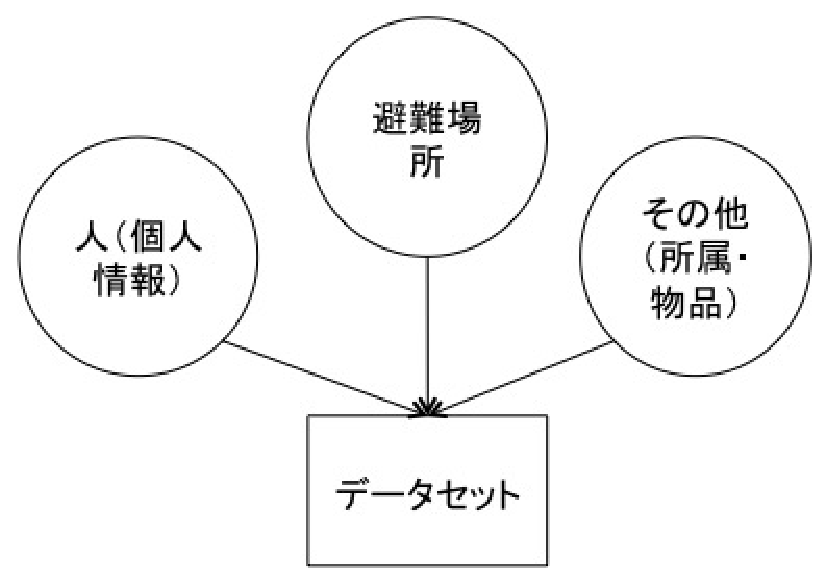
\includegraphics[width=100mm]{./images/sibm_construct.eps}
 		\caption{データセットの構成}
 		\label{fig:sibm_structrure}
 	\end{center}
\end{figure}

関係者の状況・タイプ・年齢などの情報による、所属情報などを生成される。避難場所にたいしては、収容人数情報や面積情報に対する物品情報を追加される。

避難場所情報全体には、避難場所の詳細情報と、その避難場所で避難する・作業する人たちの情報が含まれる。
避難する人や避難場所で作業する人の割合が適切に生成される(図\ref{fig:sibm_shelter})。
また、現実には、災害が発生するとき、一人以上の家族単位で避難することが考えられる。

\begin{figure}[h!]
 	\begin{center}
 		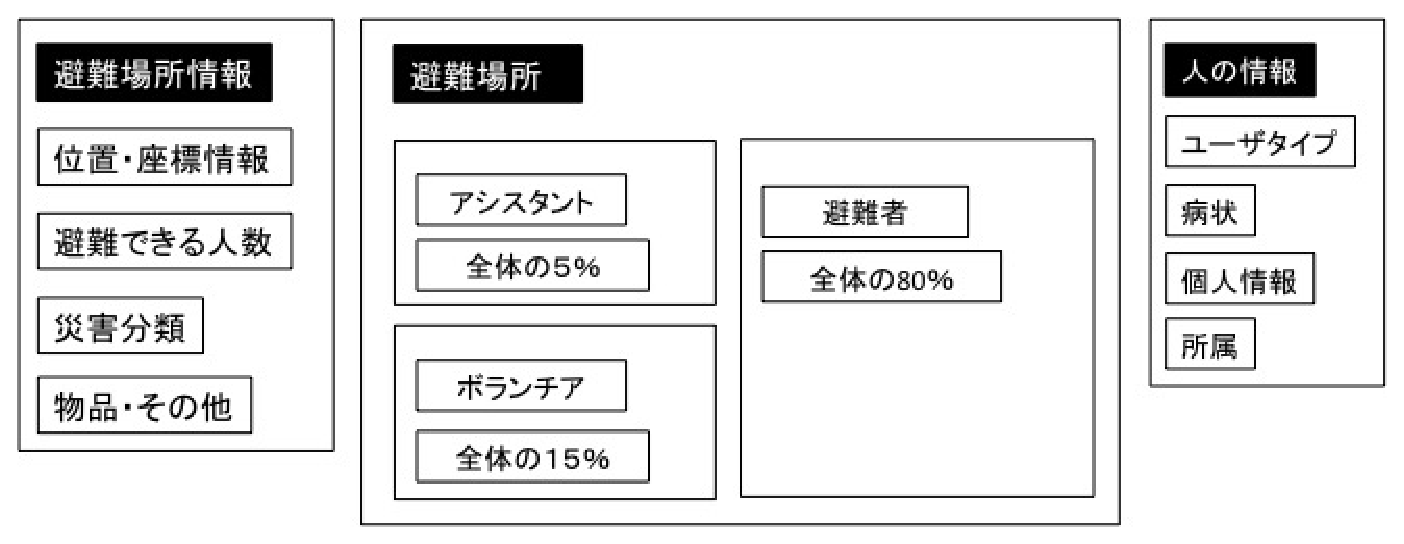
\includegraphics[width=135mm]{./images/sibm_fullimage.eps}
 		\caption{避難場所全体の構成}
 		\label{fig:sibm_shelter}
 	\end{center}
\end{figure}

また、家族全員が違う避難場所で避難することが考えあれ、SIBMでは、そのような関連を追加することが可能である(図\ref{fig:sibm_relationship})。

\begin{figure}[h!]
 	\begin{center}
 		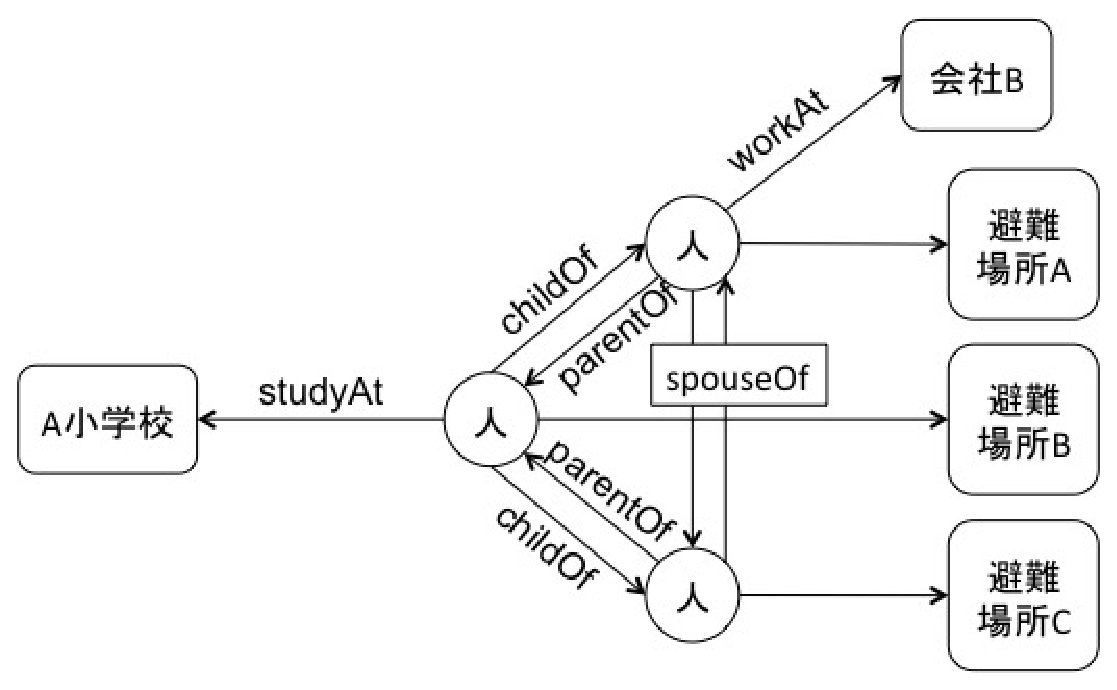
\includegraphics[width=135mm]{./images/sibm_relation.eps}
 		\caption{避難場所に置ける情報構成}
 		\label{fig:sibm_relationship}
 	\end{center}
\end{figure}

最後に、現実のように避難場所が都道府県単位で管理することを表す。
本研究では、平成24年度国土交通省による公開された全国47都道府県の避難場所情報(役12.5万箇所)を使用した。

\begin{figure}[h!]
 	\begin{center}
 		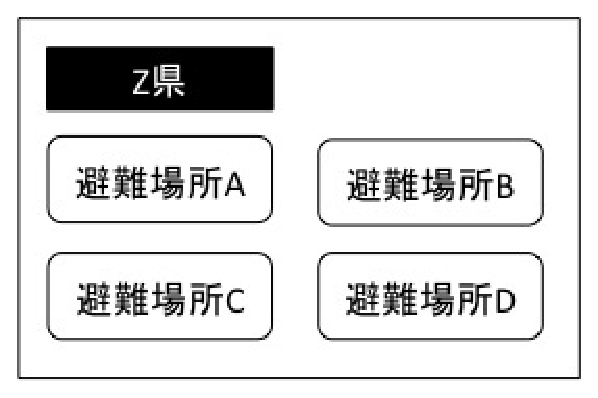
\includegraphics[width=70mm]{./images/sibm_prefecture.eps}
 		\caption{都道府県単位の避難場所構成}
 		\label{fig:sibm_prefecture}
 	\end{center}
\end{figure}

\section{SIBMの実装}
\label{sibm:implements}

\subsection{実装環境}

SIBMがApache Jena(第\ref{knowlegde:top}章)を利用して、Javaプログラミング言語で実装されている。

\subsection{データの生成}

SIBMでは、現実に近い情報を生成する目標を持ち、その目標を実装するために、実際にある情報元を使用することと、実際に近い情報を生成するツールを使用した。
上記の実装を行うための手順や関連するリソースについて以下のように説明する。

\begin{itemize}
	\item
	避難場所情報については、SIBMが\textbf{国土交通省}(MLIT\footnote{Ministry of Land, Infrastructure,
	Transport and Tourism})
	による提供した避難施設情報\footnote{http://nlftp.mlit.go.jp/ksj/index.html}を使用した
	(ただし、最新の情報ではない場合もあることから、災害時に避難施設を利用できることにならない)。
	提供した避難場所情報の詳細が(表\ref{table:data_shelter})になる。
	
	\begin{table}[h]
	\begin{center}
	\begin{tabular}{| l | l | l | p{48mm} |}
		\hline
		\rowstyle{\bfseries}
		データ項目 & フォーマット & 整備年度 & 内容 \\
		\hline
		避難施設 & 点 & 平成24年度 & 位置、行政区域、名称、住所、施設の種類、収容人数、施設規模、災害分類 \\
		\hline
	\end{tabular}
	\caption{避難場所情報の詳細}
	\label{table:data_shelter}
	\end{center}
	\end{table}
	
	また、避難場所の備蓄や、避難場所へのサポート物品・薬品などの情報が避難場所の収容人数や災害発生位置への距離による人口的に生成される。
	最後に、生成された情報をJenaによるRDFデータ形式に出力する。避難場所情報におけるRDFデータの詳細が表\ref{table:data_rdf_predicate}に表示される。
	
	\begin{table}[h]
	\begin{center}
	\begin{tabular}{| l | l | p{48mm} |}
		\hline
		\rowstyle{\bfseries}
		フィルド & RDF述語 & 内容 \\
		\hline
		位置 & geo:geopoint & 避難場所の位置 \\
		\hline
		行政区域 & sibm:administrativeAreaCode &
		都道府県コードと市区町村コードからなる、避難場所の所在する行政区を特定するためのコード \\
		\hline
		名称 & sibm:name & 避難場所の名称 \\
		\hline
		住所 & sibm:address & 避難場所の住所 \\
		\hline
		施設の種類 & sibm:facilityType & 避難場所の分類 \\
		\hline
		収容人数 & sibm:seatingCapacity & 避難施設の形態ごとの収容可能人数 \\
		\hline
		施設規模 & sibm:facilityScale & 避難施設の形態ごとの面積 \\
		\hline
		災害分類 & sibm:hazardClassification & 当該施設が対象とする災害の分類 \\
		\hline
	\end{tabular}
	\caption{避難場所情報のRDF述語の詳細}
	\label{table:data_rdf_predicate}
	\end{center}
	\end{table}

	\item
	人間の情報については、
	SIBMでは、実際の人間の個人情報ではないが、実際に近い情報を生成することができる。
	SIBMが表\ref{table:data_person}のような人間個人情報を生成するツールを構成する。
	構成したツールを使用して人間の個人情報を生成することができ、さらに複雑な情報(家族関係など)を生成することも可能である。
	
	\begin{table}[h]
	\begin{center}
	\begin{tabular}{| l | p{72mm} |}
		\hline
		\rowstyle{\bfseries}
		フィルド & 値 \\
		\hline
		firstName & NLLg \\
		\hline
		surname & Vt \\
		\hline
		gender & Female \\
		\hline
		birthday & 1982-6-5 \\
		\hline
		age & 33 \\
		\hline
		phone & +81xx-xxxx-xxxx \\
		\hline
		email & NLLg\_Vt@Caa.com \\
		\hline
		workAt & 株式会社AAzX \\
		\hline
	\end{tabular}
	\caption{個人情報の例}
	\label{table:data_person}
	\end{center}
	\end{table}
	
	ただし、生成された人中に、男女の割合や年齢の配布が日本人口構造情報による生成される。
	人は家族単位で生成され、家族の「深さ(depth)」パラメーターによる家族の人数が決められる。
	
	例えば、深さ0の家族は一人の場合にあり、3世代の家族まで検討しながら、深さ最大値は2に設定する。
	家族情報を生成する際、最小の子供の年齢から始め、日本人口の「出産平均年齢」の情報
	と「平均子供の数」の情報により、子供の数や親の年齢など家族に関する他の情報を生成する。
	
	最終的に、個人情報の中に、人の年齢、性別、タイプによる所属情報などを生成する。
	
\end{itemize}

生成された避難場所情報は基本的、ある都道府県にある避難場所のリストになり、災害発生位置から離れるような形になる。
実際では、家族の人がなるべく近い避難場所で避難するや作業することが考えられる。そのようなシナリオを実装するために、
生成された家族の人数により、避難場所リストから特定な数だけの避難場所を使用し、家族全員を特定された避難場所に
適切に分配する。

ここまで、避難場所情報・関係者情報及びそれらに関する関連情報を生成することができる。

\subsection{SPARQLクエリセット}

SIBMで生成された情報をクエリすることにより、RDFデータ管理システムを評価することができる。
ここで、第\ref{info_usage}章に説明した避難場所情報の適用シナリオにたいするクエリセットを構成する。

SIBMでは、避難場所情報だけでなく、RDFによる情報を記述したデータも扱う目的を持ち、LUBMを参考したいくつかのRDFデータ構造に対する
クエリを用意する。その一方、第\ref{info_usage}章にある使用シナリオに対するクエリセットも用意する。クエリセットの詳細は付録\ref{appendix1}
に示す。